\section{Blockchain Basics}
\subsection{The notion of \emph{block}}
In a cryptocurrecny
blockchain, like Bitcoin, a block is a proof-of-work verified set of information about a number of
transactions, the previous block in the block sequence and a nonce. The proof-of-work involves a
computation over a cryptographic puzzle. More specifically, it involves scanning for a value called
nonce, that when included in the block the total hash of the block results to a value lower than a
certain threshold.

More formally, let $G(\cdot)$, $H(\cdot)$ be cryptographic hash functions. A \textit{block} is a
triple of the form $B = \langle s, x, ctr \rangle$, where $s$ is the previous block \textit{id}, $x$
is the transactions information and $ctr \in \mathbb{N}$, such that satisfy the predicate
$validBlock^T(B)$ defined as
\begin{center}
\begin{equation}
	H(ctr, G(s,x)) < T
\end{equation}
\end{center}

The inverse of the threshold parameter $T \in \mathbb{N}$ is called the block's \textit{difficulty level}.
Throughout this work we consider a constant value for the threshold \textit{T}, although this is not
the case in a real proof-of-work blockchain.

\subsection{The notion of \emph{blockchain}}
%%%%%%%
% comment on immutability
%%%%%%%%%%%


A blockchain, or simply chain, is a timely ordered sequence of blocks.
The rightmost block is the \textit{head} the chain and is called the \textit{Genesis} block often
denoted \textit{G}, while the whole chain is denoted \textit{C}. So a chain \textit{C} with
$G = \langle s, x, ctr \rangle$ can be extended by appending a block $B = \langle s', x', ctr'
\rangle$ as long as it holds that $s' = H(ctr, G(s,x))$. In effect every block is connected to the
previous block in the chain by containing its hash. This is called the \textit{prevId} relationship.
Figure \ref{fig:abstract_chain} provides a high level representation of a blockchain including the
bootstrap step of the very first block in the chain, where instead of the \textit{prevId},
arbitrary data may be included in \textit{s}.

\begin{figure}[h!]
	\begin{center}
		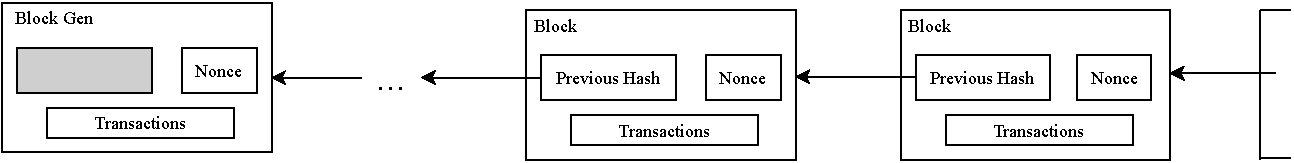
\includegraphics[scale=0.7]{figures/abstract_chain.pdf}
	\end{center}
	\caption{A high-level representation of a blockchain.}
	\label{fig:abstract_chain}
\end{figure}

Now consider a peer-to-peer network where each party may have one of the following three roles:
lightweight \textit{clients}, full \textit{nodes} and \textit{miners}.
Miners maintain an updated copy of the chain locally, while providing computational power, also
called hashpower, to extend it. In order to extend the chain by one block, the miner has to perform
a proof-of-work as already described.
Full nodes can be thought of as miners with zero hashpower. Full nodes are also called
\textit{provers}, since they provide proofs  answering the queries for specific chain information
made by clients.

\subsection{The SPV model}
Based on the Simple Payment Verification (SPV) scheme described in~\cite{nakamoto}, there can be \emph{lightweight clients}, meaning clients that need to store only the block headers of the chain. A block header includes only a Merkle Tree Root of the Merkle Tree comprised by
the transactions included in that specific block. In order to validate that a transaction is
finalized, a client needs to query the nodes until he is convinced that he has the longest
valid chain, search for the block containing that transaction and finally verify an inclusion
proof of the transaction in the block of interest.

\begin{figure}[h!]
	\begin{center}
		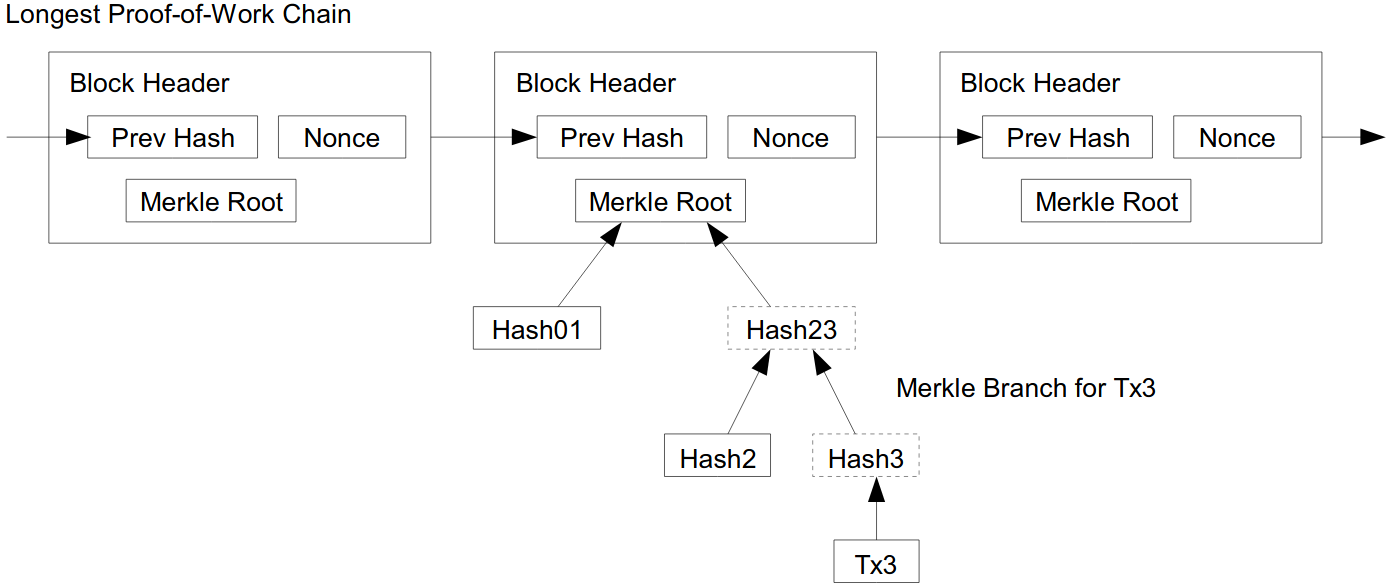
\includegraphics[scale=0.3]{figures/SPV_nakamoto.png}
	\end{center}
	\caption{High level representation of blockchain data kept by a lightweight client
	 and an inclusion proof for a transaction Tx3.\cite{nakamoto}}
	\label{fig:SPV_nakamoto}
\end{figure}

In the SPV scheme a client needs to store blockchain data of linear size to the whole chain. By
the time of writing Bitcoin's blockchain counts to almost 264GB and is estimated to grow more
than 50GB per year.  Since the growth of the chain is constantly increasing in a linear fashion, there is a need
to construct more efficient protocols serving the needs of lightweight clients. 
%Towards this end, the interaction between clients and full nodes is in our case supported  by the NIPoPoWs\cite{nipopows} primitive which allows polylogarithmic poofs to the size of the chain.